$subject$=Математическая статистика
$teacher$=Лекции Блаженова А. В.
$date$=01.04.2025

\section{Лекция 8.}

\subsection{Статистическая зависимость}

\Def Зависимость называется статистической, если изменение одной случайной величины вызывает 
изменение распределения другой.
Если при этом изменяется среднее значение другой случайной величины, то такая зависимость называется коррелеционной. 
Если при увеличении одной случайной величины среднее значение другой также увеличивается, то говорят, 
что имеет место прямая корреляция. Аналогично, если уменьшается, то -- обратная

\subsection{Корреляционное облако}

Пусть в ходе $n$ экспериментов появились значения двух случайных величин $X$ и $Y$: 

$(x_1, y_1), (x_2, y_2), \dots, (x_n, y_n)$

Нанеся точки на координатную плоскость, получаем корреляционное облако, о виде которого можно делать предположения о наличии/отсутствии связи

% https://www.geogebra.org/calculator/vjhcvrjr

\Ex 

\begin{multicols}{2}
    \begin{center}
        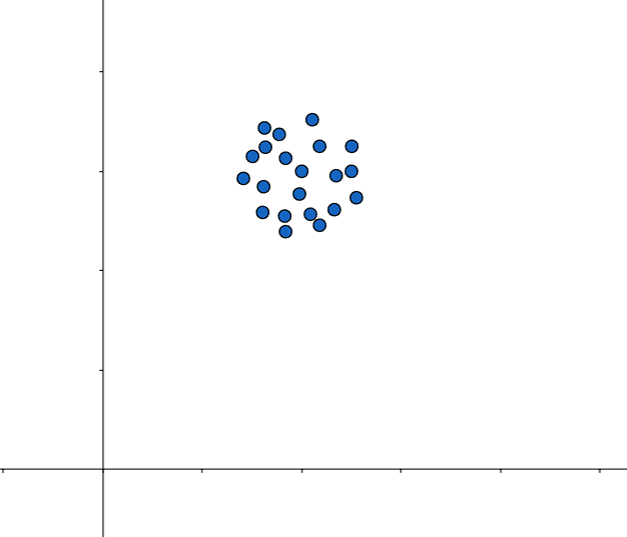
\includegraphics[height=5cm]{mathstat/images/mathstat_2025_04_01_1}

        Здесь, возможно, нет зависимости

        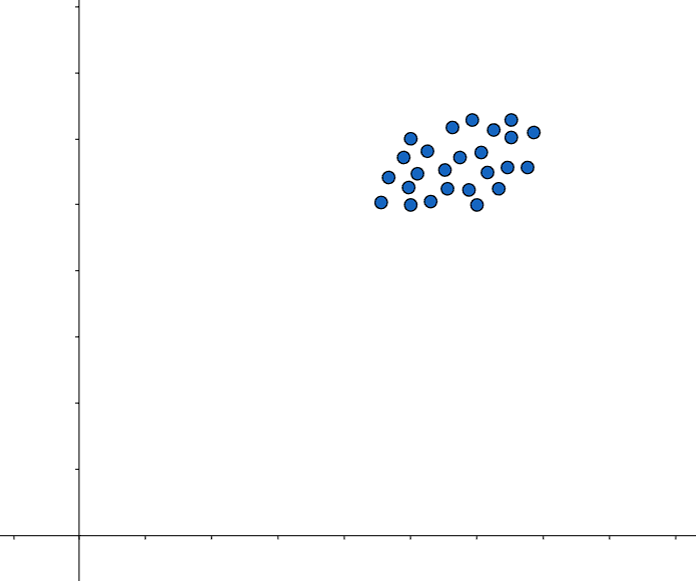
\includegraphics[height=5cm]{mathstat/images/mathstat_2025_04_01_2}

        Здесь можно предположить прямую корреляцию
    \end{center}
\end{multicols}

\subsection{Корреляционная таблица}

Пусть даны данные $X$ и $Y$ при $n$ экспериментов. Эти данные удобно представить в виде коррелеционной таблицы:
по вертикали отмечают различные значения $x$, а по горизонтали - $y$, в клетках таблицы отмечаются частота появления $n_{xy}$

\Ex $n = 50$

\smallvspace

\begin{tabular}{c|c|c|c|c|c|c}
    X\backslash Y & 10 & 20 & 30 & 40 & $n_x$ & $\overline y_x$ \\
    \hline
    2 & 7 & 3 & 0 & 0 & 10 & 13 \\
    \hline
    4 & 3 & 10 & 10 & 2 & 25 & 4.4 \\
    \hline
    6 & 0 & 2 & 10 & 3 & 15 & 30.67 \\
    \hline
    $n_y$ & 10 & 15 & 20 & 5 & $\Sigma$ 50 & \\
\end{tabular}

\smallvspace

По диагонали таблицы можно предположить, что корреляция есть

Имеет смысл вычислить условное среднее по формуле $\overline y (x) = \frac{1}{n_x} \sum n_{xy} y_i$. Так как в нашем примере
условные средние растут с ростом $x$, то имеет место прямая корреляция

\Nota Если данных много или $X$ и $Y$ -- непрерывные случайные величины, то лучше составить интервальную корреляционную таблицу:
разбить случайные величины на интервалы, по вертикали отметить интервалы $[a_{i - 1}, a_i)$ случайной величины $X$, 
по горизонтали -- $[b_{j - 1}, b_j)$ случайной величины $Y$, в клетках 
отметить частоты $n_{ij} : [a_{i - 1}, a_i) \times [b_{j - 1}, b_j)$. В дальнейшем интервалы можно заменить их серединами

\subsection{Критерий \enquote{хи-квадрат} для проверки независимости}

Пусть выборка $(X_1, Y_1), (X_2, Y_2), \dots, (X_n, Y_n)$ представлена в виде интервальной корреляционной таблицы. Случайная величина $X$ 
разбита на $k$ интервалов, а $Y$ -- на $m$ интервалов

Обозначим $v_{i\cdot}$ -- частота $i$-ого интервала $[a_{i - 1}, a_i)$ случайной величины $X$, 
$v_{\cdot j}$ -- частота $j$-ого интервала $[b_{j - 1}, b_j)$ случайной величины $Y$, $v_{ij}$ -- число точек в $[a_{i - 1}, a_i) \times [b_{j - 1}, b_j)$


\begin{tabular}{c|c|c|c|c|c}
    X\backslash Y & $[b_0, b_1)$ & $[b_1, b_2)$ & \dots & $[b_{m - 1}, b_m)$ & $v_{i\cdot}$ \\
    \hline
    $[a_0, a_1)$ & $v_{11}$ & $v_{12}$ & \dots & $v_{1m}$ & $v_{1\cdot}$ \\
    \hline
    \multicolumn{6}{c}{\dots} \\
    \hline
    $[a_{k - 1}, a_k)$ & $v_{k1}$ & $v_{k2}$ & \dots & $v_{km}$ & $v_{k\cdot}$ \\
    \hline
    $v_{\cdot j}$ & 10 & 15 & 20 & 5 & $\Sigma n$ \\
\end{tabular}

Проверяется основная гипотеза $H_0 : X \text{ и } Y$ независимы против $H_1 = \overline{H_0} : X \text{ и } Y$ зависимы

Если $H_0$ верна, то $p_{ij} = P(X \in [a_{i - 1}, a_i), Y \in [b_{j - 1}, b_j)) = P(X \in [a_{i - 1}, a_i)) \cdot P(Y \in [b_{j - 1}, b_j))$

Тогда по закону больших чисел $\frac{v_{i\cdot}}{n} \ConvergesInProbability p_{i\cdot}, \frac{v_{\cdot j}}{n} \ConvergesInProbability p_{\cdot j}$

Поэтому основанием для отклонения основной гипотезы будет заметная разница между величинами $\frac{v_{i\cdot}}{n}\frac{v_{\cdot j}}{n}$ и 
$\frac{v_{ij}}{n}$ или $v_{ij}$ и $\frac{1}{n} v_{i\cdot} v_{\cdot j}$

В качестве статистики берется $K = n \sum_{i, j} \frac{\left(v_{ij} - \frac{1}{n} v_{i\cdot} v_{\cdot j}\right)^2}{v_{i\cdot} v_{\cdot j}}$

\begin{MyTheorem}
    \Ths Если $H_0$ верна, то $K \rightrightarrows H_{(k - 1)(m - 1)}$
\end{MyTheorem}

Пусть $t_\alpha$ -- квантиль $H_{(k - 1)(m - 1)}$ уровня $\alpha$, тогда 

\begin{cases}
    H_0 : X \text{ и } Y \text{ независимы, если } K < t_\alpha \\
    H_0 : X \text{ и } Y \text{ зависимы, если } K \geq t_\alpha \\
\end{cases}

\Nota Для работы критерия необходимо, что бы частота в каждой клетке была больше 5, а объем выборки был достаточно большой

\subsection{Однофакторный дисперсионный анализ}

Предположим, что на случайную величину $X$ (результат) может влиять фактор $Z$ (необязательно, что $Z$ -- случайная величина, эксперимент может быть управляемым)

Пусть при различных \enquote{$k$ уровней} фактора $Z$ получено $k$ независимых выборок случайной величины $X$: 
$X^{(1)} = (X_1^{(1)}, \dots, X^{(1)}_{n_1}), \dots, X^{(k)} = (X_1^{(k)}, \dots, X^{(k)}_{n_k})$

Всего было получено $n = \sum_{i = 1}^k n_i$ значений

\Nota В общем говоря, распределение этих выборок отличается, поэтому эти выборки разных случайных величин

\subsubsection{Общая, внутригрупповая и межгрупповая дисперсии}

Для каждой выборки вычислим выборочное среднее и дисперсию: $\overline{x}^{(j)} = \frac{1}{n_j} \sum_{i = 1}^{n_j} X_i^{(j)}$, 
$D^{(j)} = \frac{1}{n_j} \sum_{i = 1}^{n_j} (X_i^{(j)} - \overline{x}^{(j)})^2$

Объединим все выборки в общую и также вычислим выборочнее среднее и дисперсию: 

$\overline{x} = \frac{1}{n} \sum_{i, j} x^{(j)}_i = \frac{1}{n} \sum_{j = 1}^k n_j \cdot \overline{x}^{(j)}$ - общее среднее

$D_\text{О} = \frac{1}{n} \sum_{i, j} (X^{(j)}_i - \overline{x})^2$ - общая дисперсия

\Def Внутригрупповой (или остаточной) дисперсией называется среднее групповых дисперсий: $D_{\text{В}} = \frac{1}{n} \sum_{j = 1}^k n_j D^{(j)}$

\Def Межгрупповой (или факторной) дисперсией называется величина $D_{\text{М}} = \frac{1}{n} \sum_{j = 1}^k n_j (\overline{x} - \overline{x}^{(j)})^2$

\begin{MyTheorem}
    \ThNs{О разложении дисперсии} Общая дисперсия равна сумме внутригрупповой и межгрупповой дисперсией: $D_\text{О} = D_\text{В} + D_\text{М}$
\end{MyTheorem}

Смысл: внутригрупповая дисперсия показывает средний (случайный) разброс внутри выборок, межгрупповая - насколько отличаются среднее при различных 
уровнях фактора, то есть именно эта величина отражает влияния фактора

Вывод по наличии корреляции можно сделать, если доля $D_\text{М}$ достаточно велика

\subsubsection{Проверка гипотезы о влиянии фактора}

Предполагаем, что $X$ имеет нормальное распределение и фактор $Z$ может влиять только на ее математическое ожидание, 
но на дисперсию и тип распределения, поэтому можно считать, что данные независимых $k$ выборок при различных уровнях фактора $Z$
также имеют нормальное распределение с одинаковой дисперсией: $X^{(j)} \in N(a_j, \sigma^2)$

Проверяется основная гипотеза $H_0 : a_1 = a_2 = \dots = a_k$ (фактор не оказывает влияния) против $H_1 = \overline{H_0} : $ есть влияние

По пункту 3 основной теоремы $\sum_{i = 1}^n \left(\frac{x_i - \overline{x}}{\sigma}\right)^2 = \frac{n D^*}{\sigma^2} \in H_{n - 1}$

Из этого $\frac{n_j D^{(j)}}{\sigma^2} \in H_{n_j - 1} \quad \forall \ 1 \leq j \leq k$

Так как распределение \enquote{хи-квадрат} устойчиво относительно суммирования, то $\sum_{j = 1}^k \frac{n_j D^{(j)}}{\sigma^2} \in H_{n - k}$, так как
$(n_1 - 1) + \dots + (n_k - 1) = n - k$

Пусть основная гипотеза верна, тогда все данные можно считать выборкой одной случайной величины и по пункту 3 $\frac{n D_{\text{О}}}{\sigma^2} \in H_{n - 1}$

Согласно теореме о разложении дисперсии $D_\text{О} = D_\text{В} + D_\text{М}$, тогда $\frac{n D_{\text{О}}}{\sigma^2} = \frac{n D_{\text{В}}}{\sigma^2} + \frac{n D_{\text{М}}}{\sigma^2}$

Так как $\frac{n D_{\text{О}}}{\sigma^2} \in H_{n - 1}, \frac{n D_{\text{В}}}{\sigma^2} \in H_{n - k}$, то $\frac{n D_{\text{М}}}{\sigma^2} \in H_{k - 1}$

Тогда при верной основной гипотезе получим, что $\frac{n D_{\text{М}}}{\sigma^2} \frac{\sigma^2 (n - k)}{n D_\text{В}} = \frac{n - k}{n - 1} \frac{D_\text{М}}{D_\text{В}} \in F(k - 1, n - k)$ --
распределение Фишера-Снедекера со степенями $k - 1$ и $n - k$

В качестве статистики берется $K = \frac{n - k}{n - 1} \frac{D_\text{М}}{D_\text{В}}$, в качестве критической точки $t_\alpha$ -- квантиль $F(k - 1, n - k)$ уровня $\alpha$

\begin{cases}
    H_0 : a_1 = a_2 = \dots = a_k \text{ (фактор оказывает влияние), если } K < t_\alpha \\
    H_0 : \text{фактор влияния не оказывает, если } K \geq t_\alpha \\
\end{cases}
